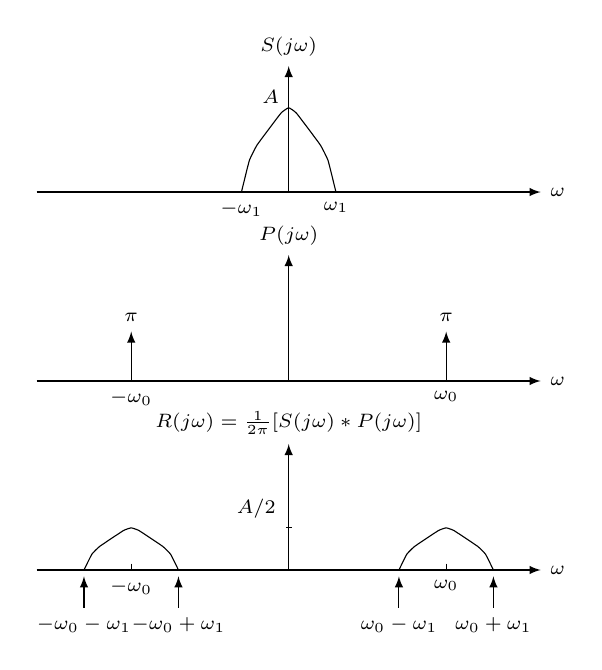
\begin{tikzpicture}[scale=0.4, every node/.append style={text=black, font=\scriptsize}]
	\begin{scope}
		\def\xmin{-8}
		\def\xmax{8}
		\def\ymin{0}
		\def\ymax{4}
		
		\draw[-latex] (\xmin, 0) -- (\xmax, 0) node[anchor=west] {$\omega$};
		\draw[-latex] (0, \ymin) -- (0, \ymax) node[anchor=south] {$S(j\omega)$};
		\node at (-1.5,0) [anchor=north] {$-\omega_1$};
		\node at (1.5,0) [anchor=north] {$\omega_1$};		
		
		\node at (0,2.5) [anchor=south east] {$A$};
		\draw  plot[smooth, tension=.2, thick, scale=0.5] coordinates {(-3,0) (-2.5,2) (-2,3) (-0.5,5) (0,5.35) (0.5, 5) (2,3) (2.5,2) (3,0)};
	\end{scope}
	
	\begin{scope}[yshift=-6cm]
		\def\xmin{-8}
		\def\xmax{8}
		\def\ymin{0}
		\def\ymax{4}
		
		\draw[-latex] (\xmin, 0) -- (\xmax, 0) node[anchor=west] {$\omega$};
		\draw[-latex] (0, \ymin) -- (0, \ymax) node[anchor=south] {$P(j\omega)$};
		\node at (-5,0) [anchor=north] {$-\omega_0$};
		\node at (5,0) [anchor=north] {$\omega_0$};		
		\draw[-latex] (-5,0) -- ++(0, pi/2) node [anchor=south] {$\pi$}; 		
		\draw[-latex] (5,0) -- ++(0, pi/2) node [anchor=south] {$\pi$}; 	
	\end{scope}
	
	\begin{scope}[yshift=-12cm]
		\def\xmin{-8}
		\def\xmax{8}
		\def\ymin{0}
		\def\ymax{4}
		
		\draw[-latex] (\xmin, 0) -- (\xmax, 0) node[anchor=west] {$\omega$};
		\draw[-latex] (0, \ymin) -- (0, \ymax) node[anchor=south] {$R(j\omega) = \frac{1}{2\pi}[S(j\omega)\ast P(j\omega)]$};
		\draw[] (-5,0.2) -- ++(0, -0.2);		
		\draw[] (5,0.2) -- ++(0, -0.2);	
		\node at (-5,0) [anchor=north] {$-\omega_0$};
		\node at (5,0) [anchor=north] {$\omega_0$};	
		\draw[latex-] (-5-1.5, -0.2) -- ++(0,-1) node[anchor=north] {$-\omega_0 - \omega_1$};
		\draw[latex-] (-5+1.5, -0.2) -- ++(0,-1) node[anchor=north] {$-\omega_0 + \omega_1$};
		\draw[latex-] (5-1.5, -0.2) -- ++(0,-1) node[anchor=north] {$\omega_0 - \omega_1$};
		\draw[latex-] (5+1.5, -0.2) -- ++(0,-1) node[anchor=north] {$\omega_0 + \omega_1$};		
		\draw  plot[smooth, tension=.2, thick, xscale=0.5, yscale=0.25, xshift= -10cm] coordinates {(-3,0) (-2.5,2) (-2,3) (-0.5,5) (0,5.35) (0.5, 5) (2,3) (2.5,2) (3,0)};
		\draw  plot[smooth, tension=.2, thick, xscale=0.5, yscale=0.25,  xshift=10cm] coordinates {(-3,0) (-2.5,2) (-2,3) (-0.5,5) (0,5.35) (0.5, 5) (2,3) (2.5,2) (3,0)};
		\draw (0.1, 5.35/4) -- ++(-0.2, 0) node [anchor=south east] {$A/2$};
	\end{scope}
	



\end{tikzpicture} 